\documentclass[11pt,a4paper]{article}
\usepackage[margin=2.2cm]{geometry}
\usepackage[T1]{fontenc}
\usepackage{lmodern}
\usepackage{microtype}
\usepackage{amsmath}
\usepackage{booktabs}
\usepackage{tabularx}
\usepackage{xcolor}
\usepackage{tikz}
\usetikzlibrary{arrows.meta,positioning,fit,backgrounds,calc}
\usepackage{pgfplots}
\pgfplotsset{compat=1.18}
\usepackage[hyphens]{url}
\usepackage{hyperref}
\usepackage{enumitem}
\setlist{nosep,leftmargin=1.4em}

\definecolor{shared}{HTML}{DBEAFE}
\definecolor{sharededge}{HTML}{1D4ED8}
\definecolor{head}{HTML}{FEF3C7}
\definecolor{headedge}{HTML}{B45309}
\definecolor{io}{HTML}{F1F5F9}
\definecolor{ioedge}{HTML}{475569}
\definecolor{cfree}{HTML}{2563EB}
\definecolor{cpro}{HTML}{D97706}
\definecolor{cent}{HTML}{059669}

\hypersetup{colorlinks=true,linkcolor=sharededge,urlcolor=sharededge}

\tikzset{
  box/.style={draw=ioedge,fill=io,rounded corners=3pt,align=center,font=\small,inner sep=5pt},
  sbox/.style={draw=sharededge,fill=shared,rounded corners=3pt,align=center,font=\small,inner sep=5pt},
  hbox/.style={draw=headedge,fill=head,rounded corners=3pt,align=center,font=\small,inner sep=5pt},
  arr/.style={-{Stealth[length=2.2mm]},thick,draw=ioedge},
}

\title{\textbf{Decide}\\[2pt]\large A sub-25\,ms typed decision engine on CPU\\shared models for routing, approval and grounding}
\author{Amal Verma}
\date{October 2026}

\begin{document}
\maketitle

\begin{abstract}
\noindent
Decide answers three typed questions about a customer-support request:
\emph{route} (one of five queues), \emph{approve} (can the action be
auto-approved) and \emph{grounded} (is the drafted reply supported by the
attached knowledge-base article). The served model is an ensemble of two
complete multi-task models, each with an encoder and a mixture of experts shared
by every decision and one linear head per decision: a fine-tuned MiniLM
cross-encoder (int8) and Ettin-17m (kept at fp32, because int8 broke it). Both
live in one 92\,MB ONNX graph and are computed in one call on CPU; their
calibrated logits are averaged, and an abstention policy is set on held-out
training data. Trained on the training split only, it scores
\textbf{85.44/100} on the public dev split with the official self-check
(classical baseline 78.45; MiniLM alone 83.75). In 4-fold cross-validation the
ensemble scored 83.13\,$\pm$\,0.53 against 82.57\,$\pm$\,1.29 for MiniLM alone,
so we expect roughly 83 to 85 on unseen data. Mean per-decision p95 latency is
20.4\,ms on a busy laptop, under the 25\,ms full-marks line.
\end{abstract}

\section{The problem, and what each question compares}

Every call names one decision and carries the full state
(\texttt{subject}, \texttt{body}, \texttt{customer\_tier}, \texttt{amount},
\texttt{draft\_reply}, \texttt{kb\_article}). The three questions are not the
same shape:

\begin{itemize}
  \item \textbf{route} reads the ticket text. It is a 5-way choice with noisy labels
        (some tickets carry two issues and the label follows the secondary one).
  \item \textbf{approve} is mostly \emph{not} a text question. Data analysis
        (Fig.~\ref{fig:approve}) shows a per-tier amount cutoff (free around \$30,
        pro around \$120, enterprise around \$500), overridden by red-flag phrases
        (``raised something similar'', ``signed up recently'', prior disputes,
        asking for an exception). A wrong approval costs three times a wrong hold.
  \item \textbf{grounded} compares two texts: does the draft change a number
        (``a quarter of an hour'' against ``an hour''), widen the scope (``all orders''
        against ``domestic orders'') or change the audience (``all users'' against
        ``administrators'')? This is natural-language inference.
\end{itemize}

\begin{figure}[h]
\centering
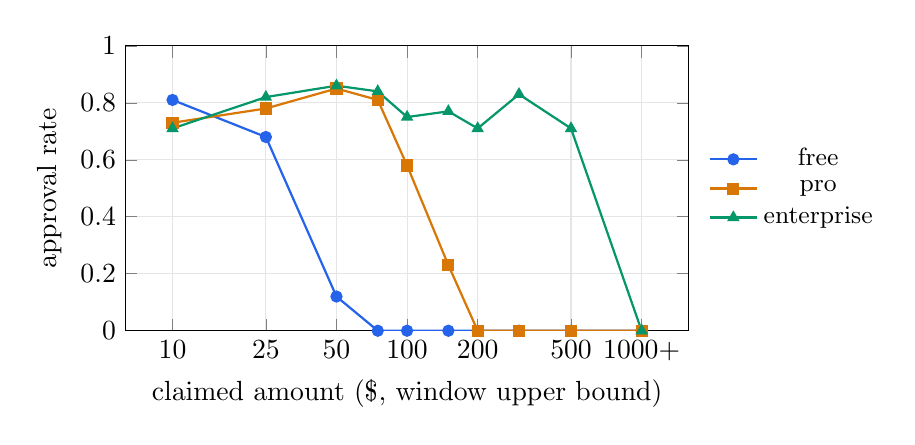
\begin{tikzpicture}
\begin{axis}[
  width=0.72\linewidth, height=5.2cm,
  xlabel={claimed amount (\$, window upper bound)}, ylabel={approval rate},
  xmode=log, log basis x=10,
  xtick={10,25,50,100,200,500,1000}, xticklabels={10,25,50,100,200,500,1000+},
  ymin=0, ymax=1, grid=major, grid style={gray!20},
  legend style={at={(1.02,0.5)},anchor=west,font=\small,draw=none},
  every axis plot/.append style={thick, mark size=1.8pt},
]
\addplot[color=cfree,mark=*] coordinates {(10,0.81)(25,0.68)(50,0.12)(75,0.0)(100,0.0)(150,0.0)(200,0.0)(300,0.0)(500,0.0)(1000,0.0)};
\addplot[color=cpro,mark=square*] coordinates {(10,0.73)(25,0.78)(50,0.85)(75,0.81)(100,0.58)(150,0.23)(200,0.0)(300,0.0)(500,0.0)(1000,0.0)};
\addplot[color=cent,mark=triangle*] coordinates {(10,0.71)(25,0.82)(50,0.86)(75,0.84)(100,0.75)(150,0.77)(200,0.71)(300,0.83)(500,0.71)(1000,0.0)};
\legend{free, pro, enterprise}
\end{axis}
\end{tikzpicture}
\caption{Approval rate by amount window and tier (train split, non-zero amounts).
Below the cutoff the rate sits near 0.8 rather than 1.0: the rest depends on red
flags and on account history the ticket does not mention, so a perfect score is not
possible.}
\label{fig:approve}
\end{figure}

\section{Architecture: where the sharing happens}

\begin{figure}[h]
\centering
\resizebox{\linewidth}{!}{%
\begin{tikzpicture}[node distance=5mm and 7mm]
  \node[box, text width=3.3cm] (r) {\textbf{route}\\(subject, body)};
  \node[box, text width=3.3cm, below=of r] (a) {\textbf{approve}\\(tier, \$amount, subject; body)\\+ tabular features};
  \node[box, text width=3.3cm, below=of a] (g) {\textbf{grounded}\\(kb\_article, draft\_reply)};

  \node[sbox, text width=2.7cm, right=14mm of r, yshift=2mm] (e1) {MiniLM-L6-H384\\encoder (int8)};
  \node[sbox, text width=2.4cm, right=6mm of e1] (m1) {gate + 4 experts\\$\sum_k g_k\,e_k$};
  \node[hbox, text width=2.3cm, right=6mm of m1] (h1) {route / approve /\\grounded heads};

  \node[sbox, text width=2.7cm, right=14mm of g, yshift=-2mm] (e2) {Ettin-17m\\encoder (fp32)};
  \node[sbox, text width=2.4cm, right=6mm of e2] (m2) {gate + 4 experts\\$\sum_k g_k\,e_k$};
  \node[hbox, text width=2.3cm, right=6mm of m2] (h2) {route / approve /\\grounded heads};

    \path let \p1=(h1.east), \p2=(a.center) in node[box, text width=2.9cm, anchor=west] (avg) at (\x1+8mm,\y2) {mean of $z_i/T_i$,\\then $/\,T_\text{final}$\\$\rightarrow$ policy};

  \draw[arr] (r.east) -- (e1.west); \draw[arr] (a.east) -- (e1.west); \draw[arr] (g.east) -- (e1.west);
  \draw[arr] (r.east) -- (e2.west); \draw[arr] (a.east) -- (e2.west); \draw[arr] (g.east) -- (e2.west);
  \draw[arr] (e1) -- (m1); \draw[arr] (m1) -- (h1);
  \draw[arr] (e2) -- (m2); \draw[arr] (m2) -- (h2);
  \draw[arr] (h1.east) -- (avg.west); \draw[arr] (h2.east) -- (avg.west);

  \begin{scope}[on background layer]
    \node[draw=sharededge, dashed, rounded corners=6pt, inner sep=6pt,
          fit=(e1)(m1)(h1)(e2)(m2)(h2),
          label={[font=\small\bfseries,text=sharededge]above:one ONNX graph, one session.run (both members)}] {};
  \end{scope}
\end{tikzpicture}}
\caption{Decide network. Inputs are framed per decision. Each member is a full
shared model: its encoder, gate and experts (blue) serve every decision; only
the final linear layer (amber) is per decision. Both members run in the same
graph and call; their temperature-scaled logits are averaged. Adding a fourth
decision means one task-embedding row and one linear head per member, plus its
training examples.}
\label{fig:arch}
\end{figure}

\paragraph{Two members, each fully shared.} Member 1 is a 6-layer, 384-wide
MiniLM cross-encoder (initialised from \path{cross-encoder/ms-marco-MiniLM-L6-v2},
Apache-2.0), pre-trained on text \emph{pairs}, which suits grounding, a
premise/hypothesis comparison. Member 2 is Ettin-17m, a 7-layer, 256-wide
encoder (\path{jhu-clsp/ettin-encoder-17m}, MIT). Each member carries its own
mixture of experts and heads and answers all three decisions; neither is
specialised. Counted from \texttt{artifacts/decide.onnx}, the members have
23.07\,M and 17.17\,M parameters (about 40.2\,M in total), of which 1{,}799 per
member are decision-specific.

\paragraph{Why Ettin stays at fp32.} Dynamic int8 quantisation leaves MiniLM
almost unchanged (int8 and fp32 give the same answer on 99.7 to 100\% of
cases) but broke Ettin: same answer on only 91\% of route, 92\% of approve and
81\% of grounded cases. The ensemble with an int8 Ettin scored 82.24 on dev;
with an fp32 Ettin, 85.44.

\paragraph{Shared mixture of experts.} Four expert MLPs ($d=256$) read the pooled
text vector, a 64-d projection of the tabular features and a 32-d task embedding.
A softmax gate over (pooled text, task embedding) mixes them. Related decisions
can reuse experts, and the differently shaped ones (approval leans on amount and
tier; grounding on pair comparison) can specialise.

\paragraph{Per-decision framing.} The approve input puts tier and amount into
the text \emph{and} supplies 75 explicit features: tier one-hots, $\log(1+\text{amount})$,
a tier $\times$ amount-cut grid at 19 cut points, and red-flag and plan-mention
indicators. A text encoder alone learns sharp numeric thresholds poorly.

\section{Training, calibration and abstention}

\begin{figure}[h]
\centering
\resizebox{\linewidth}{!}{%
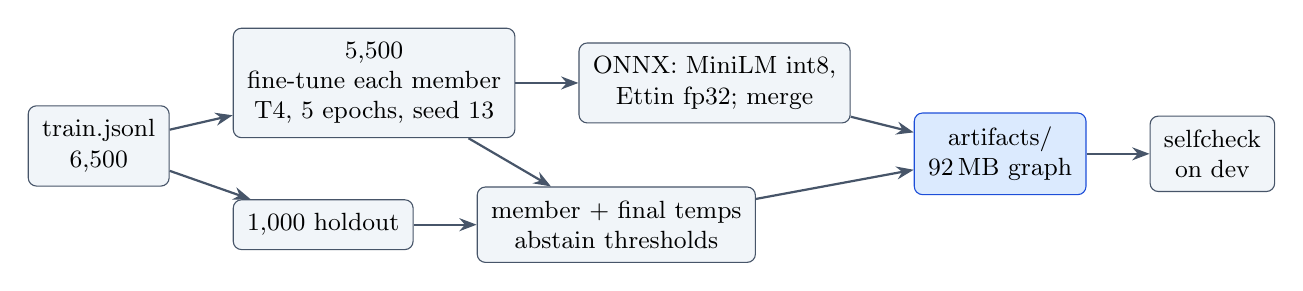
\begin{tikzpicture}[node distance=6mm and 8mm]
  \node[box] (d) {train.jsonl\\6{,}500};
  \node[box, right=of d, yshift=8mm] (tr) {5{,}500\\fine-tune each member\\T4, 5 epochs, seed 13};
  \node[box, right=of d, yshift=-10mm] (ho) {1{,}000 holdout};
  \node[box, right=of tr] (ex) {ONNX: MiniLM int8,\\Ettin fp32; merge};
  \node[box, right=of ho] (cal) {member + final temps\\abstain thresholds};
  \node[sbox, right=of ex, yshift=-9mm] (art) {artifacts/\\92\,MB graph};
  \node[box, right=of art] (sc) {selfcheck\\on dev};
  \draw[arr] (d) -- (tr); \draw[arr] (d) -- (ho);
  \draw[arr] (tr) -- (ex); \draw[arr] (ho) -- (cal); \draw[arr] (tr) -- (cal);
  \draw[arr] (ex) -- (art); \draw[arr] (cal) -- (art); \draw[arr] (art) -- (sc);
\end{tikzpicture}}
\caption{Pipeline. The dev split is never trained on; it is used for reporting.
Cross-validation (Section~\ref{sec:cv}) was used only as a consistency check and
to choose the approve abstention band.}
\end{figure}

\paragraph{Training.} Each member is trained the same way, on \texttt{train.jsonl} only with seed 13. The three decisions are trained jointly, with one decision per batch
(cross-entropy for route, binary cross-entropy for the two binaries), using AdamW
with a one-cycle schedule ($4\times10^{-5}$ encoder, $10\times$ for the new
layers), fp16, batch size 32 and max length 192. Five epochs take about 3 minutes on a T4
for MiniLM. The served Ettin member is a deterministic rerun of an earlier Ettin
run (same code, seed 13); three reruns reproduced it exactly.

\paragraph{Calibration.} Temperature scaling by negative log-likelihood on the
1{,}000-row holdout shared by both members \cite{guo2017}, in two steps
(\texttt{fit\_ensemble.py}). First one temperature per member and decision
(MiniLM: route 1.17, approve 1.03, grounded 1.22; Ettin: 1.27, 1.36, 1.15).
The scaled logits are averaged, and a final temperature is fitted on the
average: $T_\text{route}=1.00$, $T_\text{approve}=0.96$, $T_\text{grounded}=0.84$.

\paragraph{Committed value.} Approve returns ``yes'' only when $p>0.75$, the
Bayes threshold for a 3:1 cost ratio. Grounded uses $p>0.5$; route uses the arg-max.

\paragraph{Abstention.} The self-check scales quality down below 80\% coverage
and charges nothing above it, so each decision abstains on roughly its
least-confident 15\% (holdout quantiles, targeting 85\% for a margin): route
when the top probability is below 0.892, grounded when $\max(p,1-p)<0.9957$.
Approve uses a \emph{lopsided} band, abstaining when $0.15<p<0.79$: a wrong
approval costs $3\times$ a wrong hold, so confident-looking approvals are the
expensive mistakes. The band was chosen on 8{,}000 out-of-fold predictions and
kept for the ensemble (\texttt{artifacts/policy.json}).
Abstained cases still return calibrated probabilities.

\section{Results}
\subsection{Cross-validation: is dev a lucky split?}\label{sec:cv}

To check consistency, separate evaluation-only MiniLM models were trained on 4 folds
of train + dev (6{,}000 rows each, 1{,}000 of them held out for calibration and
policy). Each was scored on its 2{,}000 unseen rows with the self-check's metric
code. These fold models are not served.

\begin{table}[h]
\centering
\begin{tabular}{lc}
\toprule
 & mean $\pm$ std over 4 folds \\
\midrule
total (latency at full marks) & \textbf{82.56 $\pm$ 1.28} (83.1 / 82.9 / 83.9 / 80.5) \\
route macro-F1 & 0.940 $\pm$ 0.005 \\
approve cost (3:1) & 0.176 $\pm$ 0.017 \\
grounded macro-F1 & 0.991 $\pm$ 0.002 \\
mean ECE & 0.023 $\pm$ 0.003 \\
\bottomrule
\end{tabular}
\caption{Four-fold cross-validation. Epoch 5 beat epochs 2--4, a tuned approve
threshold gained nothing over 0.75, and a residual analysis of the 8{,}000
out-of-fold approve predictions found no learnable pattern left.}
\end{table}

MiniLM alone scored 83.75 on dev, inside this fold range. The same 4-fold test
of the ensemble idea (fresh fp32 models per fold) gave \textbf{83.13\,$\pm$\,0.53},
against 82.57\,$\pm$\,1.29 for MiniLM alone and 81.85 for Ettin alone: better
and steadier. The ensemble's dev gain (+1.69) is larger than its cross-validated
gain (+0.56), so the dev 85.44 below is partly a favourable Ettin run; an honest
hidden-test expectation is roughly 83 to 85.

\subsection{Public dev split (served model)}

All numbers come from the official \texttt{selfcheck.py} over the full dev set
(1{,}500 records $\times$ 3 decisions, one request at a time, after warm-up).
Total \textbf{85.44}: quality 0.858, calibration 0.869 (mean ECE 0.014, Brier
skill 0.81), latency 1.000, abstention 0.627; 4{,}500 of 4{,}500 responses valid.

\begin{table}[h]
\centering
\begin{tabular}{lccc}
\toprule
 & route & approve & grounded \\
\midrule
quality & macro-F1 0.947 & cost 0.179 (hold-all 0.366) & macro-F1 0.998 \\
error, full coverage & 0.107 & 0.105 & 0.012 \\
error, top 80\% by confidence & 0.051 & 0.060 & 0.001 \\
ECE & 0.014 & 0.019 & 0.010 \\
Brier score & 0.162 & 0.079 & 0.010 \\
declared coverage & 0.838 & 0.829 & 0.837 \\
p50 / p95 latency (ms) & 12.3 / 18.1 & 13.7 / 19.8 & 16.4 / 23.3 \\
\bottomrule
\end{tabular}
\caption{Served ensemble (MiniLM int8 + Ettin-17m fp32), public dev split.
Latency measured on a busy laptop (load average 3.5 to 4.5).}
\end{table}

\begin{table}[h]
\centering
\begin{tabular}{lc}
\toprule
model (same self-check, trained on train only) & total \\
\midrule
classical baseline & 78.45 \\
MiniLM + Ettin-17m, Ettin int8 & 82.24 \\
MiniLM + Ettin-17m, a different Ettin run & 82.78 \\
MiniLM H384 + MoE alone (mean p95 10.7\,ms) & 83.75 \\
Ettin-17m + MoE alone, fp32 (approve coverage 0.790) & 84.68 \\
\textbf{MiniLM + Ettin-17m, Ettin fp32 (served)} & \textbf{85.44} \\
\bottomrule
\end{tabular}
\caption{Dev totals of the alternatives.}
\end{table}

\begin{figure}[h]
\centering
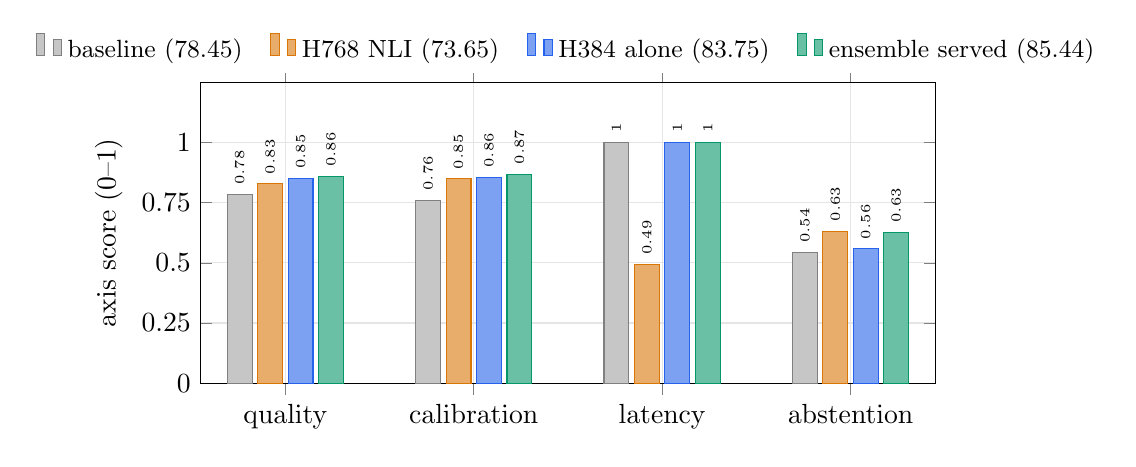
\begin{tikzpicture}
\begin{axis}[
  ybar, bar width=9pt, width=0.9\linewidth, height=5.4cm,
  symbolic x coords={quality,calibration,latency,abstention},
  xtick=data, ymin=0, ymax=1.25, ytick={0,0.25,0.5,0.75,1}, ylabel={axis score (0--1)},
  legend style={at={(0.5,1.03)},anchor=south,legend columns=4,font=\small,draw=none,/tikz/every even column/.append style={column sep=8pt}},
  nodes near coords, every node near coord/.append style={font=\tiny,rotate=90,anchor=west},
  enlarge x limits=0.15, grid=major, grid style={gray!20},
]
\addplot[fill=gray!45,draw=gray] coordinates {(quality,0.783)(calibration,0.760)(latency,1.0)(abstention,0.542)};
\addplot[fill=cpro!60,draw=cpro] coordinates {(quality,0.828)(calibration,0.849)(latency,0.492)(abstention,0.632)};
\addplot[fill=cfree!60,draw=cfree] coordinates {(quality,0.850)(calibration,0.856)(latency,1.0)(abstention,0.558)};
\addplot[fill=cent!60,draw=cent] coordinates {(quality,0.858)(calibration,0.869)(latency,1.0)(abstention,0.627)};
\legend{baseline (78.45), H768 NLI (73.65), H384 alone (83.75), ensemble served (85.44)}
\end{axis}
\end{tikzpicture}
\caption{Score axes (weights: quality 40\%, calibration 25\%, latency 20\%,
abstention 15\%). The H768 run used an earlier coverage target of 82\%, under which its
grounded coverage fell to 0.75, below the 80\% target.}
\label{fig:scores}
\end{figure}

Latency was measured on a laptop i5-1135G7 (8 threads) with ONNX Runtime pinned to 4
intra-op threads. Latency depends on machine load. The ensemble's mean p95 was
20.4\,ms with load average 3.5 to 4.5, and 23.0\,ms in a fresh-venv run of
\texttt{scripts/verify\_submission.sh} under similar load: full marks, but with
less headroom than MiniLM alone (10.7\,ms). In Fig.~\ref{fig:scores} the H384 bar comes from a quiet run;
the H768 bar was measured under heavy unrelated load (load average about 13),
where H384 itself measured 37\,ms. So the H768 latency bar is pessimistic, but
it was about $1.7\times$ slower than H384 under identical load.

\section{Trade-offs}

\paragraph{Ensemble over one model.} The ensemble costs about twice the latency
of MiniLM alone, but gained +1.69 on dev and +0.56 in cross-validation, with a
smaller spread across folds, and still gets full latency marks.

\paragraph{H384 over H768.}

We trained the same multi-task model on two backbones. The larger
\path{cross-encoder/nli-MiniLM2-L6-H768} (NLI pre-trained) grounds perfectly
on dev (F1 1.000 against 0.991) but runs about $1.7\times$ slower. Its mean p95 was
63\,ms against 37\,ms under identical load, which costs half of the 20\% latency
axis. A 0.009 F1 gain on one of three decisions does not pay for that, so we
serve H384.

\section{Where it fails}

\begin{itemize}
  \item \textbf{Routing}: about 11\% of dev labels disagree with the evident topic,
        mostly multi-issue tickets. Probabilities spread out on these instead of
        claiming certainty; route ECE is 0.014.
  \item \textbf{Approval}: errors cluster at the tier cutoffs and on cases decided by
        account history the ticket never mentions. The error rate at full
        coverage is 10.5\%; on the 80\% the model is most confident about, it is 6.0\%.
  \item \textbf{Grounding}: it catches changed numbers well, but hand-written
        drafts that invent an action (``I have put yours through'') or narrow
        the scope (``only on the enterprise plan'') were scored as grounded.
  \item \textbf{Latency}: on a heavily loaded host the ensemble's p95 can pass 25\,ms.
  \item The data is synthetic and templated. Unseen phrasing, other currencies or
        new tiers will degrade it, and the amount features assume USD-scale values.
\end{itemize}

\section{Reproducing}

\begin{tabularx}{\linewidth}{@{}l>{\raggedright\arraybackslash}X@{}}
Serve & \texttt{pip install -r requirements.txt \&\& uvicorn app:app -{}-host 0.0.0.0 -{}-port 8000} \\
Score & \texttt{python selfcheck.py -{}-url http://localhost:8000/v1/decide} \\
Train & \texttt{kaggle/decide\_train.ipynb} on a Kaggle T4, or \texttt{train\_encoder.py} on any GPU \\
Policy & \texttt{python fit\_ensemble.py <ensemble dir> data/train.jsonl} \\
\end{tabularx}

\paragraph{Pretrained components.} \path{cross-encoder/ms-marco-MiniLM-L6-v2}
(Apache-2.0, served member 1), \path{jhu-clsp/ettin-encoder-17m} (MIT, served
member 2) and \path{cross-encoder/nli-MiniLM2-L6-H768} (Apache-2.0, compared
only). Libraries: PyTorch, Transformers, ONNX Runtime, tokenizers,
FastAPI, Uvicorn, scikit-learn, LightGBM.

\begin{thebibliography}{9}
\bibitem{guo2017} C.~Guo, G.~Pleiss, Y.~Sun, K.~Q.~Weinberger.
  \emph{On Calibration of Modern Neural Networks.} ICML 2017.
\end{thebibliography}

\end{document}
